\documentclass[11pt,a4paper]{article}

\usepackage[utf8]{inputenc}
\usepackage[T1]{fontenc}
\usepackage[margin=2cm, headheight=15pt]{geometry}
\usepackage{graphicx}
\usepackage{xcolor}
\usepackage{amsmath,amssymb}
\usepackage{booktabs}
\usepackage{array}
\usepackage{hyperref}
\usepackage{fancyhdr}

% Palette de couleurs
\definecolor{inptblue}{HTML}{1E40AF}
\definecolor{inptlight}{HTML}{EFF6FF}
\definecolor{hackergreen}{HTML}{008833}
\definecolor{slate}{HTML}{334155}
\definecolor{amber}{HTML}{B45309}

\hypersetup{
    colorlinks=true,
    linkcolor=inptblue,
    urlcolor=inptblue,
    pdftitle={Guide Pedagogique et Cours de Reseau - IPv4 Subnet Toolkit v1.2.0},
    pdfauthor={INPT - Cursus Ingenieur ASEDS}
}

% En-tete et pied de page
\pagestyle{fancy}
\fancyhf{}
\fancyhead[L]{\small\textbf{\textcolor{inptblue}{IPv4 Subnet Toolkit v1.2.0}} — Guide Applicatif \& Cours}
\fancyhead[R]{\small\textcolor{slate}{INPT — ASEDS}}
\fancyfoot[C]{\thepage}

\setlength{\parskip}{0.55em}
\setlength{\parindent}{0pt}

% Boite pedagogique personnalisee (sans dependance externe complexe)
\newcommand{\coursbox}[2]{%
    \vspace{0.4em}
    \noindent\fcolorbox{inptblue}{inptlight}{%
        \parbox{\dimexpr\linewidth-2\fboxsep-2\fboxrule\relax}{%
            \textbf{\textcolor{inptblue}{#1}}\\[0.3em]
            #2
        }%
    }%
    \vspace{0.4em}
}

\begin{document}

% ============================================================================
% PAGE DE TITRE
% ============================================================================
\begin{titlepage}
    \centering
    \vspace*{1.5cm}
    {\Large \textbf{\textcolor{inptblue}{INSTITUT NATIONAL DES POSTES ET TÉLÉCOMMUNICATIONS (INPT)}}}\\[0.3cm]
    {\large Cursus Ingénieur — Filière ASEDS}\\[2cm]

    \rule{\linewidth}{0.6mm}\\[0.5cm]
    {\Huge \textbf{\textcolor{inptblue}{IPv4 Subnet Toolkit v1.2.0}}}\\[0.4cm]
    {\LARGE \textbf{Manuel Pédagogique de l'Application \& Raisonnement Complet du Cours de Réseau IPv4}}\\[0.3cm]
    \rule{\linewidth}{0.6mm}\\[1.2cm]

    {\large \textit{Comprendre le rôle de chaque composant de l'interface graphique, la méthodologie de résolution visuelle et les fondements mathématiques du cours (Adressage, Masques, Sous-Réseaux, VLSM, Fragmentation MTU, Routage LPM \& Checksum 16 bits).}}\\[1.5cm]

    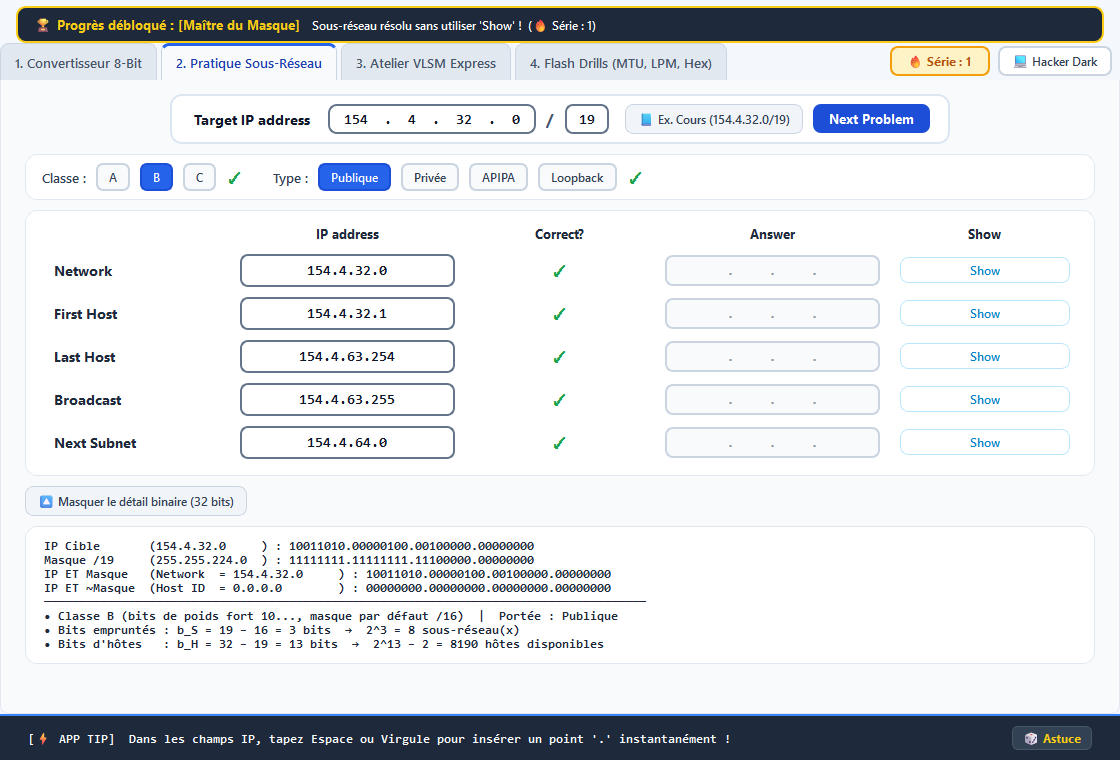
\includegraphics[width=0.92\textwidth]{../screenshots/03_tab2_subnet_solved_drawer_light.png}\\[1.2cm]

    \vfill
    {\large \textbf{Version 1.2.0 — Octobre 2026}}\\
    {\normalsize Document de référence illustré par les captures d'écran réelles de l'application}
\end{titlepage}

\tableofcontents
\newpage

% ============================================================================
% CHAPITRE 1 : PHILOSOPHIE & ERGONOMIE COGNITIVE
% ============================================================================
\section{Philosophie Pédagogique : Pourquoi l'Application est Conçue Ainsi}

Lorsqu'on prépare les examens et travaux dirigés de \textbf{Réseaux Informatiques (IPv4)} en cycle ingénieur, deux obstacles majeurs ralentissent l'apprentissage :
\begin{enumerate}
    \item \textbf{La fatigue mécanique (Surcharge Cognitive)} : Dans un exercice de découpage VLSM classique, calculer 3 ou 4 sous-réseaux oblige à écrire 18 à 24 adresses IP complètes (Réseau, Masque, 1er Hôte, Dernier Hôte, Broadcast). Au bout de deux exercices, l'étudiant passe 80\,\% de son temps à recopier des octets répétitifs au lieu d'entraîner sa prise de décision mathématique.
    \item \textbf{L'opacité du calcul binaire sur 32 bits} : Les calculatrices IP en ligne donnent directement la réponse finale sans montrer \textit{comment} l'opérateur logique \texttt{ET} (\texttt{AND}) ou le complément à un (\texttt{$\sim$Masque}) agissent bit par bit.
\end{enumerate}

Pour résoudre ces deux problèmes, \textbf{IPv4 Subnet Toolkit v1.2.0} repose sur quatre piliers ergonomiques visibles partout dans l'application :

\subsection{Pilier 1 — « Tester la Décision, Automatiser la Répétition »}
Dans l'atelier VLSM (Onglet 3), l'application vous demande uniquement le \textbf{cœur mathématique} :
\begin{itemize}
    \item Quel besoin traiter en premier ? (\textit{Tri décroissant}).
    \item Quel préfixe \texttt{/CIDR} choisir ? (\textit{Loi des puissances de 2 : $2^h - 2 \ge N$}).
    \item Quelle est la nouvelle \textbf{Adresse Réseau} ? (\textit{Addition du pas $2^h$}).
\end{itemize}
Dès que ces 3 décisions sont exactes ($\checkmark$), l'application \textbf{auto-complète instantanément} la plage d'hôtes utilisables (\texttt{First Host $\to$ Last Host}), l'adresse de \texttt{Broadcast} et le masque décimal !

\subsection{Pilier 2 — La Divulgation Progressive (Tiroir Binaire 32-Bit)}
Dans l'onglet 2 (\textit{Pratique Sous-Réseau}), le détail binaire sur 32 bits est placé dans un tiroir repliable (\texttt{Afficher le détail binaire (32 bits)}), fermé par défaut. Cela vous entraîne d'abord à calculer vite de tête (grâce au \textit{Magic Number}), tout en vous permettant d'ouvrir le tiroir à tout moment pour vérifier les opérations bit à bit du cours (\texttt{IP ET Masque}, \texttt{IP ET $\sim$Masque}, bits empruntés $b_S$ et bits d'hôtes $b_H$).

\subsection{Pilier 3 — Saisie Clavier Ultra-Rapide (\texttt{IpLineEdit} Smart Auto-Dot)}
Tous les champs d'adresse IP de l'application utilisent un composant intelligent :
\begin{itemize}
    \item Appuyer sur \textbf{Espace} ou \textbf{Virgule} insère immédiatement un point \texttt{.} (ou saute par-dessus un point existant).
    \item Taper \textbf{3 chiffres} (ex: \texttt{192}) insère automatiquement le point \texttt{.}.
    \item \textbf{Nouveauté v1.2.0 (Auto-Dot $\ge 26$)} : Puisqu'un octet IPv4 ne peut jamais dépasser \texttt{255}, \textbf{aucun octet valide à 3 chiffres ne peut commencer par un nombre entre 26 et 99} (car $260 > 255$). Dès que vous tapez 2 chiffres supérieurs ou égaux à 26 (ex: \texttt{32}, \texttt{68}, \texttt{99}), l'application insère le point \texttt{.} toute seule sans attendre !
\end{itemize}

\subsection{Pilier 4 — Répétition Espacée \& Gamification Style Minecraft}
\begin{itemize}
    \item \textbf{Bannière d'astuces en bas de fenêtre} : Toutes les 12 secondes (ou au clic sur \texttt{Astuce}), une règle fondamentale du cours INPT s'affiche (\texttt{[COURS INPT]}, \texttt{[ASTUCE PRO]}, \texttt{[APP TIP]}).
    \item \textbf{Compteur de Série \& Succès} : En haut à droite, le badge \texttt{Série : X} s'incrémente chaque fois que vous résolvez un exercice complet \textbf{sans avoir cliqué sur le bouton d'aide \texttt{Show}}, débloquant des bannières de progrès (\textit{Maître du Masque}, \textit{Architecte VLSM}, \textit{Chirurgien MTU}, \textit{Routeur Humain}, \textit{Seigneur du Checksum}).
\end{itemize}

\newpage
% ============================================================================
% CHAPITRE 2 : ONGLET 1 — CONVERTISSEUR 8-BIT & INSPECTEUR DE MASQUE
% ============================================================================
\section{Onglet 1 — Convertisseur Binaire 8-Bit \& Inspecteur de Masque}

\begin{figure}[!htbp]
    \centering
    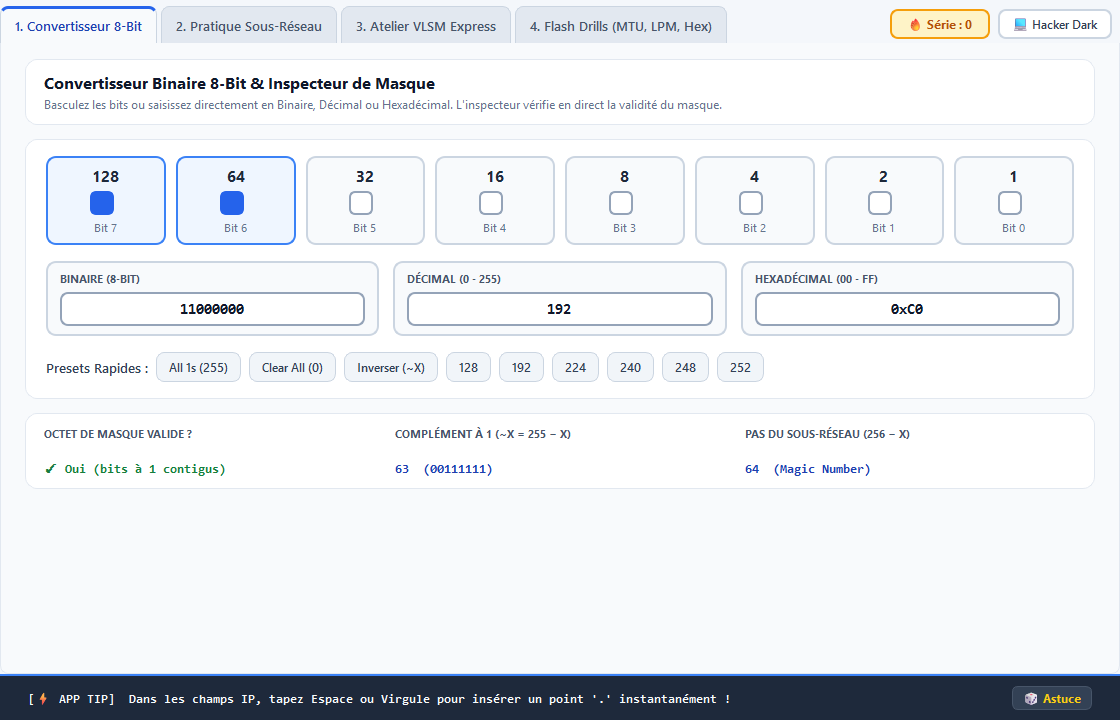
\includegraphics[width=0.95\textwidth]{../screenshots/01_tab1_mask_valid_light.png}
    \caption{Onglet 1 en Mode Clair : l'octet \texttt{192} (\texttt{11000000}) est reconnu comme un octet de masque valide avec un pas (Magic Number) de \texttt{64}.}
\end{figure}

\subsection{Pourquoi chaque élément est présent sur cet écran}
\begin{enumerate}
    \item \textbf{Les 8 Cartes de Bits (\texttt{128, 64, 32, 16, 8, 4, 2, 1})} :
    Un octet IPv4 est un entier non signé sur 8 bits ($b_7 b_6 b_5 b_4 b_3 b_2 b_1 b_0$) dont la valeur décimale est :
    $$V = \sum_{i=0}^{7} b_i \cdot 2^i = 128 b_7 + 64 b_6 + 32 b_5 + 16 b_4 + 8 b_3 + 4 b_2 + 2 b_1 + 1 b_0$$
    Cliquer sur les cases permet de visualiser immédiatement comment les puissances de 2 s'additionnent.
    \item \textbf{Synchronisation Temps Réel à 3 Voies (Binaire / Décimal / Hexadécimal)} :
    Utile à la fois pour l'adressage IPv4 (décimal/binaire) et pour le calcul de Checksum d'en-tête ou d'analyse Wireshark (hexadécimal \texttt{0x00} à \texttt{0xFF}).
    \item \textbf{Les Presets Rapides (\texttt{128, 192, 224, 240, 248, 252})} :
    Ce sont les valeurs d'octets de masque que vous rencontrerez dans 99\,\% des exercices de sous-réseaux et de VLSM.
\end{enumerate}

\subsection{Le Raisonnement du Cours : L'Inspecteur de Masque \& Complément}
En bas de l'onglet 1, la barre \textbf{Inspecteur de Masque \& Complément} enseigne trois notions fondamentales du cours :

\subsubsection{1. Qu'est-ce qu'un Octet de Masque Valide ? (Règle de Contiguïté)}
Dans le cours de réseau, un masque de sous-réseau sert à séparer la \textbf{partie Réseau} (à gauche, bits à \texttt{1}) de la \textbf{partie Hôte} (à droite, bits à \texttt{0}).
\textbf{Règle absolue} : Les bits à \texttt{1} d'un masque doivent être \textbf{strictement contigus} en partant du bit de poids fort (Bit 7 = 128). Il est interdit d'avoir un \texttt{0} suivi d'un \texttt{1}.

Il n'existe donc que \textbf{9 valeurs décimales possibles} pour un octet de masque :
\begin{center}
\begin{tabular}{@{}cccc@{}}
\toprule
\textbf{Bits à 1} & \textbf{Binaire (8 bits)} & \textbf{Valeur Décimale ($X$)} & \textbf{Pas du Sous-Réseau ($256 - X$)} \\
\midrule
0 bit  & \texttt{00000000} & \textbf{0}   & 256 \\
1 bit  & \texttt{10000000} & \textbf{128} & 128 \\
2 bits & \texttt{11000000} & \textbf{192} & 64  \\
3 bits & \texttt{11100000} & \textbf{224} & 32  \\
4 bits & \texttt{11110000} & \textbf{240} & 16  \\
5 bits & \texttt{11111000} & \textbf{248} & 8   \\
6 bits & \texttt{11111100} & \textbf{252} & 4   \\
7 bits & \texttt{11111110} & \textbf{254} & 2   \\
8 bits & \texttt{11111111} & \textbf{255} & 1   \\
\bottomrule
\end{tabular}
\end{center}

\begin{figure}[!htbp]
    \centering
    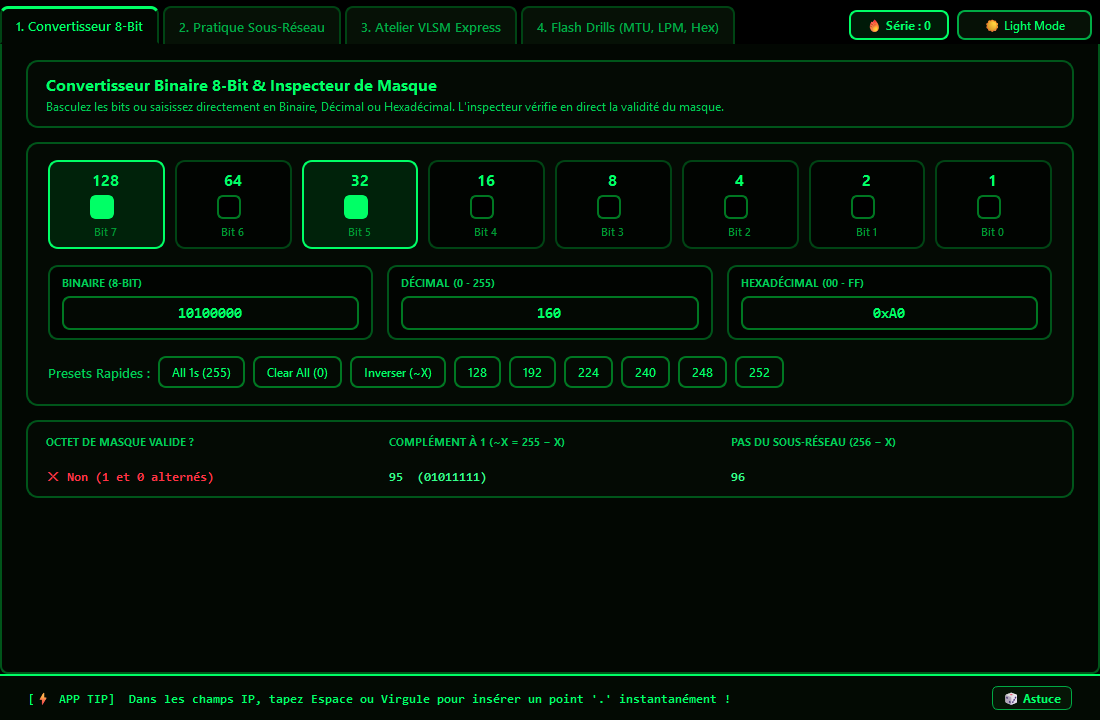
\includegraphics[width=0.95\textwidth]{../screenshots/02_tab1_mask_invalid_hacker.png}
    \caption{Onglet 1 en Mode Hacker Dark : l'octet \texttt{170} (\texttt{10101010}) alterne des \texttt{1} et des \texttt{0} $\to$ l'inspecteur indique immédiatement \texttt{Non (1 et 0 alternés)}.}
\end{figure}

\subsubsection{2. Le Complément à 1 ($\sim X = 255 - X$)}
Le complément à un inverse tous les bits (\texttt{0 $\leftrightarrow$ 1}). Arithmétiquement, puisque la somme de tous les bits vaut $255$ (\texttt{11111111}), inverser les bits revient à calculer :
$$\sim X = 255 - X$$
Sur la capture \texttt{192} (\texttt{11000000}), le complément à un vaut $255 - 192 = 63$ (\texttt{00111111}). Dans le cours, ce complément est utilisé pour :
\begin{itemize}
    \item Extraire le \textbf{Host ID Interne} d'une machine via $\text{IP} \ \text{ET} \ (\sim\text{Masque})$.
    \item Calculer l'adresse de \textbf{Broadcast} via $\text{Network} \ \text{OU} \ (\sim\text{Masque})$ (c'est-à-dire additionner $\sim X$ à l'octet réseau ! Ex: $0 + 63 = 63$, $64 + 63 = 127$).
\end{itemize}

\subsubsection{3. Le Pas du Sous-Réseau (\textit{Magic Number} = $256 - X$)}
Le pas $256 - X$ donne l'espacement exact entre deux sous-réseaux consécutifs dans l'octet où le masque s'arrête. Avec $X = 192$, le pas vaut $256 - 192 = 64$ : les sous-réseaux commencent donc aux multiples de 64 (\texttt{.0}, \texttt{.64}, \texttt{.128}, \texttt{.192}).

\newpage
% ============================================================================
% CHAPITRE 3 : ONGLET 2 — PRATIQUE SOUS-RESEAU & TIROIR BINAIRE 32 BITS
% ============================================================================
\section{Onglet 2 — Pratique Sous-Réseau, Classes \& Tiroir Binaire 32-Bit}

\begin{figure}[!htbp]
    \centering
    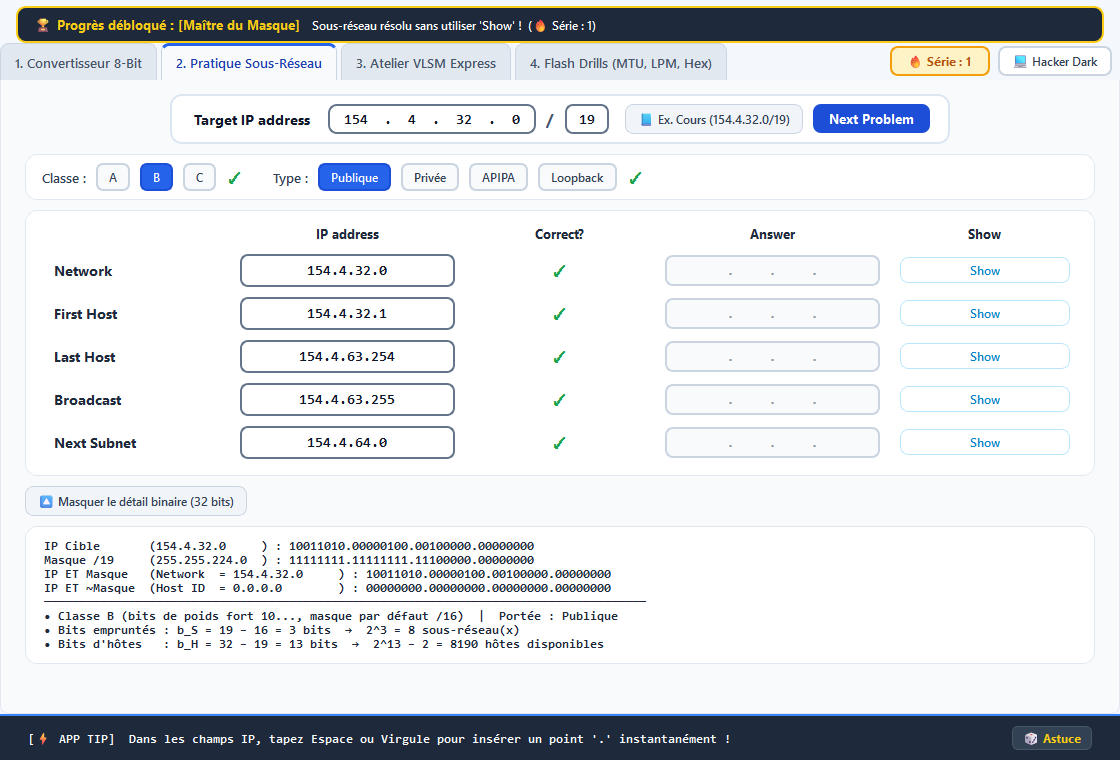
\includegraphics[width=0.95\textwidth]{../screenshots/03_tab2_subnet_solved_drawer_light.png}
    \caption{Onglet 2 avec l'exercice officiel du cours (\texttt{154.4.32.0/19}) entièrement résolu, le tiroir binaire 32 bits déployé et la bannière de succès débloquée.}
\end{figure}

\subsection{Pourquoi la Barre de Classification (Classe \& Type) est Placée en Haut}
Avant même de calculer les plages d'un sous-réseau, le cours de réseau demande toujours de qualifier l'adresse IP cible selon deux axes :

\coursbox{Rappel du Cours INPT — Classes d'Adresses IPv4 (1er Octet)}{
\begin{itemize}
    \item \textbf{Classe A} : \texttt{0} à \texttt{127} (Bit de poids fort \texttt{0...}, masque par défaut \textbf{\texttt{/8}} soit \texttt{255.0.0.0}).
    \item \textbf{Classe B} : \texttt{128} à \texttt{191} (Bits de poids fort \texttt{10...}, masque par défaut \textbf{\texttt{/16}} soit \texttt{255.255.0.0}).
    \item \textbf{Classe C} : \texttt{192} à \texttt{223} (Bits de poids fort \texttt{110...}, masque par défaut \textbf{\texttt{/24}} soit \texttt{255.255.255.0}).
    \item \textbf{Classe D} : \texttt{224} à \texttt{239} (Bits \texttt{1110...}, réservée au \textbf{Multicast} / diffusion de groupe).
    \item \textbf{Classe E} : \texttt{240} à \texttt{255} (Bits \texttt{11110...}, réservée pour un usage futur / expérimental).
\end{itemize}
}

\coursbox{Rappel du Cours INPT — Portée \& Types d'Adresses Spéciales}{
\begin{itemize}
    \item \textbf{Privée (RFC 1918)} — Non routable sur Internet (nécessite du NAT) :
    \begin{itemize}
        \item Classe A : \texttt{10.0.0.0/8} (\texttt{10.0.0.0} à \texttt{10.255.255.255})
        \item Classe B : \texttt{172.16.0.0/12} (\texttt{172.16.0.0} à \texttt{172.31.255.255} — 16 réseaux de classe B)
        \item Classe C : \texttt{192.168.0.0/16} (\texttt{192.168.0.0} à \texttt{192.168.255.255} — 256 réseaux de classe C)
    \end{itemize}
    \item \textbf{Loopback (Boucle locale)} : \texttt{127.0.0.0/8} (ex: \texttt{127.0.0.1} pour tester la pile TCP/IP locale).
    \item \textbf{APIPA} : \texttt{169.254.0.0/16} (attribuée automatiquement par l'OS quand aucun serveur DHCP ne répond).
    \item \textbf{Publique} : Toute autre adresse unicast routable sur Internet (comme \texttt{154.4.32.0} sur la capture ci-dessus).
\end{itemize}
}

\subsection{Résolution Détaillée de l'Exemple du Cours (\texttt{154.4.32.0/19})}
Regardons comment le tableau à 5 lignes et le tiroir binaire 32 bits (Figure 3) résolvent l'exemple officiel du cours :
\begin{enumerate}
    \item \textbf{Identification de la Classe} : Le 1er octet est \texttt{154}. Comme $128 \le 154 \le 191$ (en binaire \texttt{10011010}, commence par \texttt{10}), c'est une \textbf{Classe B} (masque par défaut \texttt{/16}) et elle n'appartient pas à \texttt{172.16.0.0/12} ni \texttt{169.254.0.0/16} $\implies$ \textbf{Publique}.
    \item \textbf{Analyse du Masque \texttt{/19}} :
    $$\text{19 bits à 1} = \underbrace{11111111}_{255}.\underbrace{11111111}_{255}.\underbrace{11100000}_{224}.\underbrace{00000000}_{0} \implies \texttt{255.255.224.0}$$
    L'octet « intéressant » est le \textbf{3ème octet} (valeur $224$). Son pas (\textit{Magic Number}) vaut $256 - 224 = 32$.
    \item \textbf{Calcul des 5 lignes du tableau} :
    \begin{itemize}
        \item \textbf{Network Address} : Dans le 3ème octet, le multiple de $32$ inférieur ou égal à $32$ est $32$ lui-même $\implies$ \textbf{\texttt{154.4.32.0}}.
        \item \textbf{Next Subnet} : On ajoute le pas de $32$ au 3ème octet : $32 + 32 = 64 \implies$ \textbf{\texttt{154.4.64.0}}.
        \item \textbf{Broadcast Address} : Dernière adresse juste avant \texttt{154.4.64.0} $\implies$ \textbf{\texttt{154.4.63.255}}.
        \item \textbf{First Host} : $\text{Network} + 1 \implies$ \textbf{\texttt{154.4.32.1}}.
        \item \textbf{Last Host} : $\text{Broadcast} - 1 \implies$ \textbf{\texttt{154.4.63.254}}.
    \end{itemize}
    \item \textbf{Lecture du Tiroir Binaire 32-Bit (en bas de la Figure 3)} :
    \begin{itemize}
        \item \textbf{Bits empruntés ($b_S$)} : Par rapport au masque par défaut \texttt{/16} de la Classe B, on a emprunté $b_S = 19 - 16 = 3$ bits à la partie hôte, ce qui permet de créer $2^3 = \mathbf{8}$ \textbf{sous-réseaux}.
        \item \textbf{Bits d'hôtes ($b_H$)} : Il reste $b_H = 32 - 19 = 13$ bits à \texttt{0} pour les machines, soit $2^{13} - 2 = 8192 - 2 = \mathbf{8190}$ \textbf{hôtes disponibles} par sous-réseau.
        \item \textbf{Host ID Interne} : Calculé par $\text{IP} \ \text{ET} \ (\sim\text{Masque})$. Ici, comme l'IP cible \texttt{154.4.32.0} est déjà l'adresse réseau, tous ses bits hôtes sont à \texttt{0} (\texttt{0.0.0.0}). Si l'IP cible était \texttt{154.4.35.12}, son Host ID interne serait \texttt{0.0.3.12}.
    \end{itemize}
\end{enumerate}

\begin{figure}[!htbp]
    \centering
    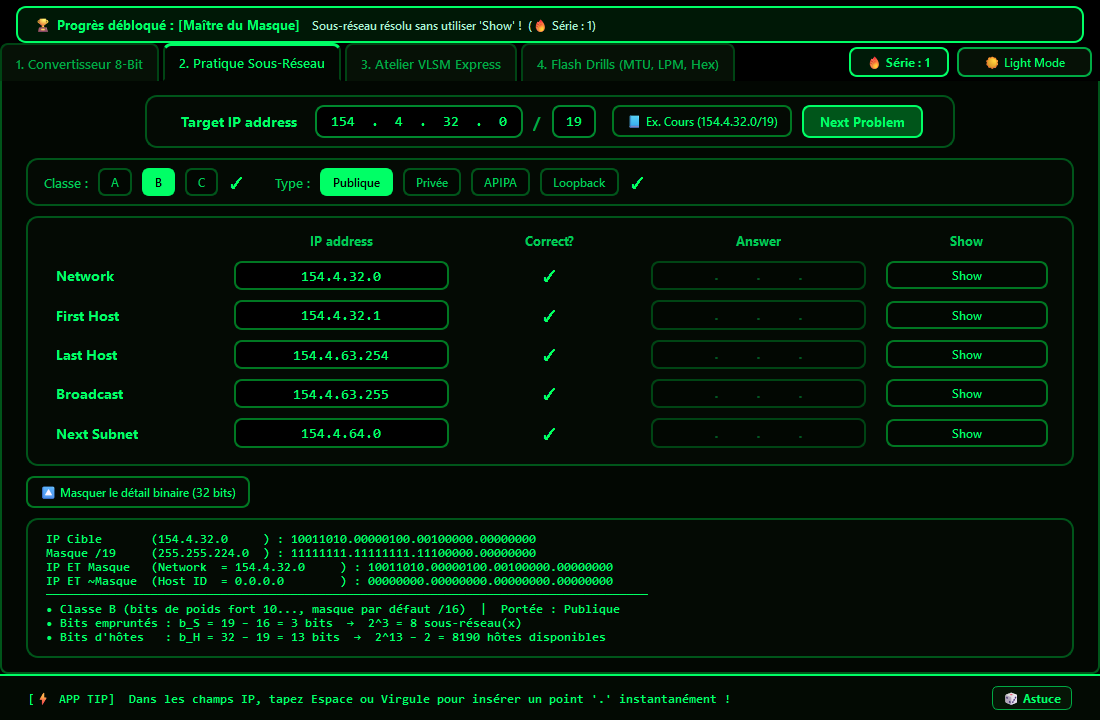
\includegraphics[width=0.92\textwidth]{../screenshots/04_tab2_subnet_hacker.png}
    \caption{Onglet 2 en thème \textbf{Hacker Dark} (\texttt{\#000000} / \texttt{\#00FF66}) inspiré des terminaux réseau.}
\end{figure}

\newpage
% ============================================================================
% CHAPITRE 4 : ONGLET 3 — ATELIER VLSM EXPRESS
% ============================================================================
\section{Onglet 3 — Atelier VLSM Express (Découpage à Masque Variable)}

\begin{figure}[!htbp]
    \centering
    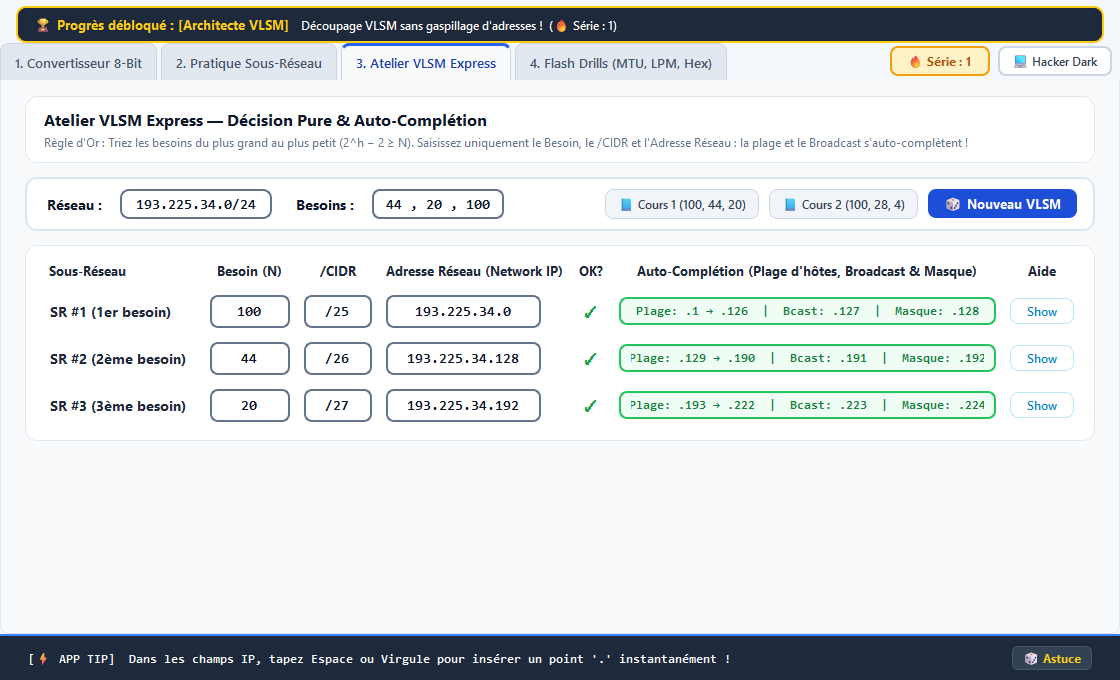
\includegraphics[width=0.95\textwidth]{../screenshots/05_tab3_vlsm_cours1_solved_light.png}
    \caption{Onglet 3 — Résolution de l'Exercice Officiel du Cours 1 (\texttt{193.225.34.0/24} pour \texttt{44, 20, 100} machines) avec auto-complétion verte des plages.}
\end{figure}

\subsection{Pourquoi le Découpage Classique (FLSM) ne Suffit Pas}
En découpage fixe (\textit{Fixed Length Subnet Mask}), tous les sous-réseaux ont la même taille. Si un service a besoin de 100 machines (\texttt{/25}, 126 places) et qu'une liaison point-à-point ou un petit bureau n'a besoin que de 4 machines, lui attribuer aussi un \texttt{/25} gaspille $126 - 4 = 122$ adresses IP !
Le \textbf{VLSM (\textit{Variable Length Subnet Mask})} résout ce problème en adaptant la longueur du masque \texttt{/CIDR} à chaque besoin réel.

\subsection{Les 3 Étapes Mathématiques Testées par l'Onglet 3}
\begin{enumerate}
    \item \textbf{Colonne 1 — \texttt{Besoin (N)} (Le Tri Décroissant Obligatoire)} :
    Dans la barre du haut (Figure 5), les besoins sont donnés en désordre : \texttt{44 , 20 , 100}.
    Vous devez impérativement les saisir du \textbf{plus grand au plus petit} (\texttt{100}, puis \texttt{44}, puis \texttt{20}).
    \textit{Pourquoi ?} Parce qu'en binaire, un sous-réseau de taille $2^h$ doit toujours démarrer sur une adresse multiple de $2^h$. En plaçant les plus grands blocs en premier ($\text{Pas } 128 \to \text{Pas } 64 \to \text{Pas } 32$), chaque sous-réseau est naturellement aligné sur sa frontière binaire sans jamais chevaucher le précédent !
    \item \textbf{Colonne 2 — \texttt{/CIDR} (Loi de dimensionnement $2^h - 2 \ge N$)} :
    Pour $N$ machines, on cherche la plus petite puissance $h$ telle que :
    $$2^h - 2 \ge N \quad \text{(soit } 2^h \ge N + 2\text{ en comptant Réseau et Broadcast)}$$
    Puis on déduit :
    $$\text{CIDR} = 32 - h \quad \text{et} \quad \text{Pas (Taille du bloc)} = 2^h$$
    \item \textbf{Colonne 3 — \texttt{Adresse Réseau (Network IP)}} :
    Le 1er sous-réseau démarre à l'adresse de base. Le sous-réseau suivant démarre à :
    $$\text{Network}_{k+1} = \text{Network}_k + 2^{h_k}$$
\end{enumerate}

\subsection{Corrigé Complet des 2 Exercices Officiels du Cours INPT}

\subsubsection{Exercice du Cours 1 : Réseau \texttt{193.225.34.0/24} — Besoins \texttt{[44, 20, 100]} (Figure 5)}
\begin{center}
\resizebox{\linewidth}{!}{%
\begin{tabular}{@{}ccccccc@{}}
\toprule
\textbf{Rang} & \textbf{Besoin $N$} & \textbf{Calcul $2^h - 2 \ge N$} & \textbf{/CIDR} & \textbf{Masque} & \textbf{Adresse Réseau} & \textbf{Plage Hôtes \& Broadcast} \\
\midrule
SR \#1 & \textbf{100} & $2^7 - 2 = 126 \ge 100$ ($h=7$, Pas=128) & \textbf{/25} & \texttt{.128} & \textbf{\texttt{193.225.34.0}}   & \texttt{.1 $\to$ .126} | Bcast \texttt{.127} \\
SR \#2 & \textbf{44}  & $2^6 - 2 = 62 \ge 44$ ($h=6$, Pas=64)   & \textbf{/26} & \texttt{.192} & \textbf{\texttt{193.225.34.128}} & \texttt{.129 $\to$ .190} | Bcast \texttt{.191} \\
SR \#3 & \textbf{20}  & $2^5 - 2 = 30 \ge 20$ ($h=5$, Pas=32)   & \textbf{/27} & \texttt{.224} & \textbf{\texttt{193.225.34.192}} & \texttt{.193 $\to$ .222} | Bcast \texttt{.223} \\
\bottomrule
\end{tabular}%
}
\end{center}
\textit{Adresses restantes non allouées} : de \texttt{193.225.34.224} à \texttt{.255} (soit 32 adresses libres).

\begin{figure}[!htbp]
    \centering
    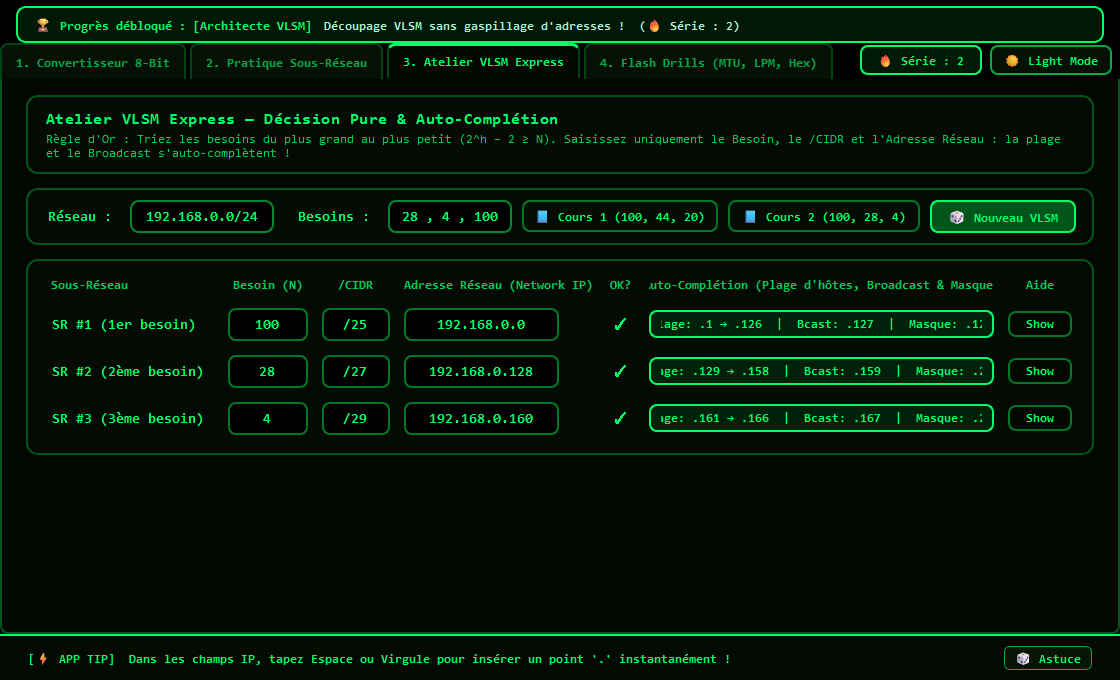
\includegraphics[width=0.95\textwidth]{../screenshots/06_tab3_vlsm_cours2_hacker.png}
    \caption{Onglet 3 en Mode Hacker Dark — Résolution de l'Exercice Officiel du Cours 2 (\texttt{192.168.0.0/24} pour \texttt{100, 28, 4} machines).}
\end{figure}

\subsubsection{Exercice du Cours 2 : Réseau \texttt{192.168.0.0/24} — Besoins \texttt{[100, 28, 4]} (Figure 6)}
\begin{center}
\resizebox{\linewidth}{!}{%
\begin{tabular}{@{}ccccccc@{}}
\toprule
\textbf{Rang} & \textbf{Besoin $N$} & \textbf{Calcul $2^h - 2 \ge N$} & \textbf{/CIDR} & \textbf{Masque} & \textbf{Adresse Réseau} & \textbf{Plage Hôtes \& Broadcast} \\
\midrule
SR \#1 & \textbf{100} & $2^7 - 2 = 126 \ge 100$ ($h=7$, Pas=128) & \textbf{/25} & \texttt{.128} & \textbf{\texttt{192.168.0.0}}   & \texttt{.1 $\to$ .126} | Bcast \texttt{.127} \\
SR \#2 & \textbf{28}  & $2^5 - 2 = 30 \ge 28$ ($h=5$, Pas=32)   & \textbf{/27} & \texttt{.224} & \textbf{\texttt{192.168.0.128}} & \texttt{.129 $\to$ .158} | Bcast \texttt{.159} \\
SR \#3 & \textbf{4}   & $2^3 - 2 = 6 \ge 4$ ($h=3$, Pas=8)      & \textbf{/29} & \texttt{.248} & \textbf{\texttt{192.168.0.160}} & \texttt{.161 $\to$ .166} | Bcast \texttt{.167} \\
\bottomrule
\end{tabular}%
}
\end{center}

\newpage
% ============================================================================
% CHAPITRE 5 : ONGLET 4 — FLASH DRILLS (MTU, ROUTAGE LPM & CHECKSUM)
% ============================================================================
\section{Onglet 4 — Flash Drills : Fragmentation MTU, Routage LPM \& Checksum}

Pour éviter de surcharger l'écran, l'onglet 4 dispose d'une barre de sélection en haut qui permet de basculer entre les \textbf{3 grands exercices classiques d'examen} du cours de réseau.

\subsection{Mini-Exercice 1 : Fragmentation IPv4 \& MTU}

\begin{figure}[!htbp]
    \centering
    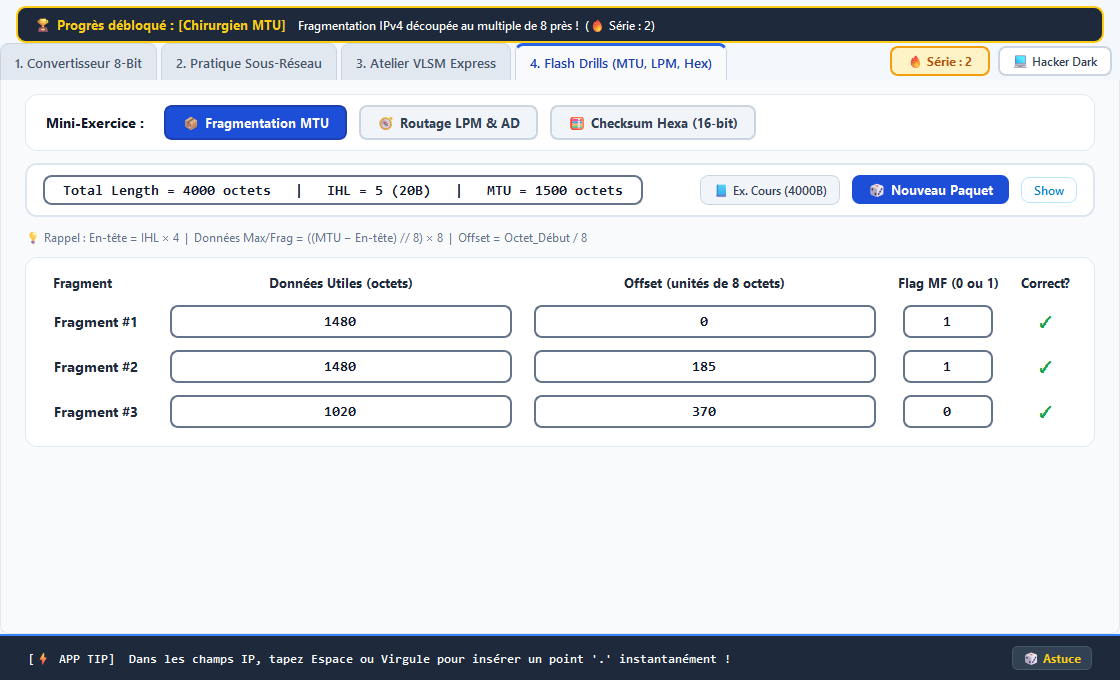
\includegraphics[width=0.95\textwidth]{../screenshots/07_tab4_drill_mtu_solved.png}
    \caption{Onglet 4 (Vue 1) — Exercice officiel de Fragmentation MTU (\texttt{Total Length = 4000 octets}, \texttt{IHL = 5}, \texttt{MTU = 1500 octets}).}
\end{figure}

\subsubsection{Le Raisonnement Mathématique du Cours}
Lorsqu'un routeur doit transmettre un paquet IPv4 de taille totale \texttt{Total Length} sur une liaison dont la taille maximale de trame est \texttt{MTU} (\textit{Maximum Transmission Unit}, typiquement 1500 octets sur Ethernet), si $\text{Total Length} > \text{MTU}$, le paquet doit être découpé en plusieurs fragments IPv4 :
\begin{enumerate}
    \item \textbf{Taille de l'En-Tête (\texttt{Header Length})} : Le champ \texttt{IHL} indique le nombre de mots de 32 bits (4 octets) de l'en-tête.
    $$L_{\text{en-tête}} = \text{IHL} \times 4 \quad (\text{Ex: } \text{IHL}=5 \implies 20\text{ octets})$$
    \textit{Important} : Chaque fragment créé recevra sa propre copie de cet en-tête de 20 octets !
    \item \textbf{Données Originales à Transporter} :
    $$D_{\text{initial}} = \text{Total Length} - L_{\text{en-tête}} = 4000 - 20 = 3980\text{ octets}$$
    \item \textbf{Données Utiles Max par Fragment (Règle du Multiple de 8)} :
    Dans l'en-tête IPv4, le champ \texttt{Fragment Offset} est codé sur 13 bits alors que la longueur totale est sur 16 bits ($2^{16} / 2^{13} = 8$). L'Offset compte donc par \textbf{blocs de 8 octets}. Par conséquent, la quantité de données de chaque fragment (sauf le dernier) \textbf{doit être divisible par 8} :
    $$D_{\max} = \left\lfloor \frac{\text{MTU} - L_{\text{en-tête}}}{8} \right\rfloor \times 8 = \left\lfloor \frac{1500 - 20}{8} \right\rfloor \times 8 = 185 \times 8 = 1480\text{ octets}$$
    \item \textbf{Calcul des 3 Colonnes de la Figure 7} :
    \begin{itemize}
        \item \textbf{Fragment \#1} : Transporte \textbf{1480} octets de données (octets $0$ à $1479$). Début = octet $0 \implies \text{Offset} = 0 / 8 = \mathbf{0}$. Il reste $3980 - 1480 = 2500$ octets $\implies$ bit \textbf{MF (\textit{More Fragments}) = 1}.
        \item \textbf{Fragment \#2} : Transporte \textbf{1480} octets de données (octets $1480$ à $2959$). Début = octet $1480 \implies \text{Offset} = 1480 / 8 = \mathbf{185}$. Il reste $2500 - 1480 = 1020$ octets $\implies$ \textbf{MF = 1}.
        \item \textbf{Fragment \#3} : Transporte les \textbf{1020} derniers octets (octets $2960$ à $3979$). Début = octet $2960 \implies \text{Offset} = 2960 / 8 = \mathbf{370}$. C'est le dernier fragment $\implies$ \textbf{MF = 0}.
    \end{itemize}
\end{enumerate}

\newpage
\subsection{Mini-Exercice 2 : Table de Routage, Longest Prefix Match (LPM) \& AD}

\begin{figure}[!htbp]
    \centering
    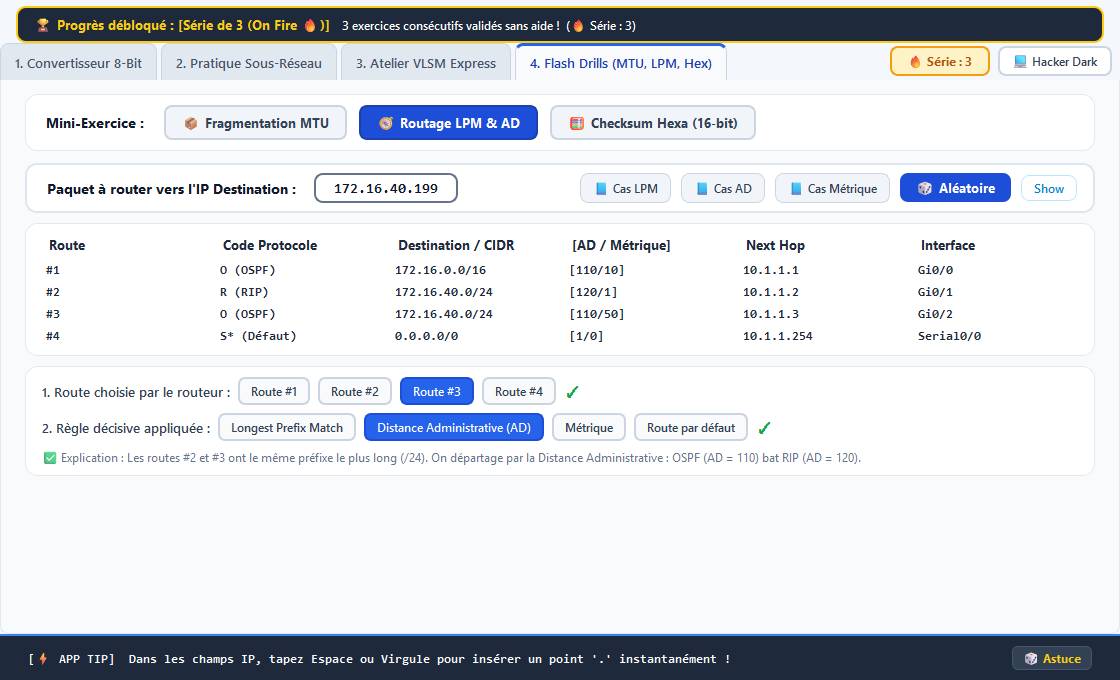
\includegraphics[width=0.95\textwidth]{../screenshots/08_tab4_drill_lpm_solved.png}
    \caption{Onglet 4 (Vue 2) — Table de routage et sélection de la route gagnante et de la règle décisive.}
\end{figure}

\subsubsection{L'Algorithme Exact de Sélection de Route d'un Routeur IP}
Pour acheminer un paquet vers une adresse \texttt{IP Destination} (ex: \texttt{172.16.30.74} sur la Figure 8), le routeur n'examine jamais les routes au hasard. Il applique un filtre suivi de \textbf{3 règles hiérarchiques strictes} :
\begin{enumerate}
    \item \textbf{Étape 0 — Filtrage d'Appartenance} : Le routeur élimine toutes les lignes de la table dont le préfixe réseau ne contient pas l'IP de destination.
    \textit{Piège classique d'examen présent dans l'application} : Si une route est en \texttt{192.168.10.0/26} (qui ne couvre que \texttt{.0} à \texttt{.63}) et que le paquet va vers \texttt{192.168.10.80}, cette route \texttt{/26} ne correspond \textbf{pas} !
    \item \textbf{Règle 1 — Longest Prefix Match (LPM / Plus Long Préfixe)} :
    Parmi toutes les routes qui correspondent à l'IP de destination, le routeur choisit \textbf{toujours celle qui possède le masque \texttt{/CIDR} le plus grand} (la route la plus spécifique : \texttt{/26 > /24 > /16 > /8 > /0}), quelle que soit sa distance administrative !
    \item \textbf{Règle 2 — Distance Administrative (AD)} :
    Si (et seulement si) plusieurs routes correspondantes ont \textbf{exactement le même préfixe \texttt{/CIDR} le plus long}, le routeur départage selon la fiabilité du protocole (plus petite AD gagne) :
    \begin{center}
    \begin{tabular}{@{}lcc@{}}
    \toprule
    \textbf{Protocole / Origine de la Route} & \textbf{Code Table} & \textbf{Distance Administrative (AD)} \\
    \midrule
    Réseau Directement Connecté & \texttt{C}  & \textbf{0}   \\
    Route Statique              & \texttt{S}  & \textbf{1}   \\
    OSPF (état de liens)        & \texttt{O}  & \textbf{110} \\
    RIP (vecteur de distance)   & \texttt{R}  & \textbf{120} \\
    \bottomrule
    \end{tabular}
    \end{center}
    Sur la Figure 8, les routes \#2 (\texttt{R 172.16.30.0/24 [120/1]}) et \#3 (\texttt{O 172.16.30.0/24 [110/50]}) ont le même masque \texttt{/24}. Même si RIP affiche une métrique de \texttt{1} contre \texttt{50} pour OSPF, le routeur compare d'abord l'\textbf{AD} : $\text{OSPF (110)} < \text{RIP (120)} \implies$ \textbf{Route \#3 gagne par Distance Administrative} !
    \item \textbf{Règle 3 — Métrique} :
    Si plusieurs routes ont le \textbf{même \texttt{/CIDR}} et la \textbf{même AD} (même protocole), le routeur choisit la plus petite métrique.
    \item \textbf{Cas de la Route par Défaut (\texttt{0.0.0.0/0}, \texttt{S*})} :
    Son masque est \texttt{/0} (0 bit vérifié : elle correspond à 100\,\% des adresses IPv4, mais avec le préfixe le plus court possible). Elle n'est donc utilisée que si aucune autre route de la table ne correspond à la destination.
\end{enumerate}

\newpage
\subsection{Mini-Exercice 3 : Somme de Contrôle de l'En-tête IPv4 (Checksum 16-Bit)}

\begin{figure}[!htbp]
    \centering
    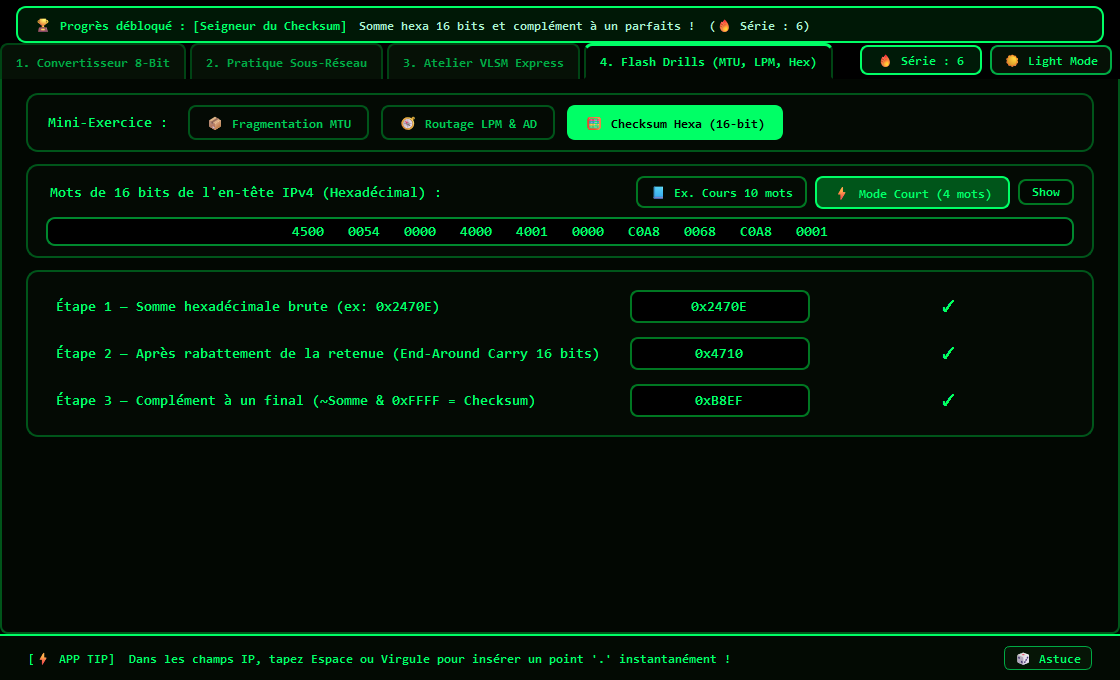
\includegraphics[width=0.95\textwidth]{../screenshots/09_tab4_drill_checksum_solved.png}
    \caption{Onglet 4 (Vue 3) en Mode Hacker Dark — Calcul en 3 étapes du Checksum 16 bits sur l'exemple officiel du cours.}
\end{figure}

\subsubsection{Pourquoi et Comment Calculer le Checksum IPv4 (Figure 9)}
L'en-tête IPv4 (20 octets pour $\text{IHL}=5$) contient un champ \texttt{Header Checksum} de 16 bits qui protège l'en-tête contre les erreurs de transmission et qui doit être recalculé à chaque routeur (car le champ \texttt{TTL} diminue de 1 à chaque saut).

Le cours décompose ce calcul en \textbf{3 étapes}, exactement reproduites par les 3 champs de saisie de la Figure 9 :
\begin{enumerate}
    \item \textbf{Étape 1 — Somme Hexadécimale Brute des 10 Mots de 16 Bits} :
    On place le champ Checksum (6ème mot) à \texttt{0000} et on additionne les mots de 16 bits :
    $$\texttt{4500} + \texttt{0054} + \texttt{0000} + \texttt{4000} + \texttt{4001} + \texttt{0000} + \texttt{C0A8} + \texttt{0068} + \texttt{C0A8} + \texttt{0001} = \mathbf{\texttt{0x2470E}}$$
    \item \textbf{Étape 2 — Rabattement de la Retenue (\textit{End-Around Carry} sur 16 bits)} :
    Le résultat \texttt{0x2470E} dépasse 16 bits (4 chiffres hexa). Le chiffre de dépassement à gauche est \texttt{2} (poids $2 \times 2^{16}$). On l'additionne aux 16 bits de droite (\texttt{0x470E}) :
    $$\texttt{0x470E} + \texttt{0x0002} = \mathbf{\texttt{0x4710}}$$
    \item \textbf{Étape 3 — Complément à Un Final ($\sim\text{Somme} \ \& \ \texttt{0xFFFF}$)} :
    On inverse tous les bits (ou de manière équivalente en hexadécimal, on soustrait chaque chiffre à \texttt{F}, soit $\texttt{0xFFFF} - \texttt{0x4710}$) :
    $$\begin{array}{cccccc}
      & \texttt{F} & \texttt{F} & \texttt{F} & \texttt{F} \\
    - & \texttt{4} & \texttt{7} & \texttt{1} & \texttt{0} \\
    \hline
    = & \mathbf{\texttt{B}} & \mathbf{\texttt{8}} & \mathbf{\texttt{E}} & \mathbf{\texttt{F}}
    \end{array}
    \implies \text{Checksum final} = \mathbf{\texttt{0xB8EF}}$$
\end{enumerate}
\textit{Vérification par le récepteur} : À la réception du paquet, le routeur additionne les 10 mots \textbf{en incluant} le Checksum \texttt{0xB8EF}. Après rabattement de la retenue, il obtient $\texttt{0x4710} + \texttt{0xB8EF} = \texttt{0xFFFF}$ (que des \texttt{1}, dont le complément à un vaut \texttt{0x0000}), preuve que l'en-tête est intact !

\end{document}
